\documentclass[
11pt, % The default document font size, options: 10pt, 11pt, 12pt
oneside, % Two side (alternating margins) for binding by default, uncomment to switch to one side
%chapterinoneline,% Have the chapter title next to the number in one single line
english, % ngerman for German
singlespacing, % Single line spacing, alternatives: onehalfspacing or doublespacing
%draft, % Uncomment to enable draft mode (no pictures, no links, overfull hboxes indicated)
%nolistspacing, % If the document is onehalfspacing or doublespacing, uncomment this to set spacing in lists to single
%liststotoc, % Uncomment to add the list of figures/tables/etc to the table of contents
%toctotoc, % Uncomment to add the main table of contents to the table of contents
%parskip, % Uncomment to add space between paragraphs
%nohyperref, % Uncomment to not load the hyperref package
headsepline, % Uncomment to get a line under the header
]{MastersDoctoralThesis} % The class file specifying the document structure

\usepackage[utf8]{inputenc} % Required for inputting international characters
\usepackage[T1]{fontenc} % Output font encoding for international characters

\usepackage{palatino} % Use the Palatino font by default

\usepackage[backend=bibtex,style=authoryear,natbib=true]{biblatex} % Use the bibtex backend with the authoryear citation style (which resembles APA)

\addbibresource{example.bib} % The filename of the bibliography

\usepackage[autostyle=true]{csquotes} % Required to generate language-dependent quotes in the bibliography

\usepackage[cm-default]{fontspec}
\usepackage{enumerate}

\setromanfont{FreeSerif}
\setsansfont{FreeSans}
\setmonofont{FreeMono}

\usepackage{xltxtra} 
\usepackage{xgreek} 

\usepackage{amsmath}

\usepackage{ragged2e}

\usepackage{float}
%----------------------------------------------------------------------------------------
%	MARGIN SETTINGS
%----------------------------------------------------------------------------------------

\geometry{
	paper=a4paper, % Change to letterpaper for US letter
	inner=2.5cm, % Inner margin
	outer=3.8cm, % Outer margin
	bindingoffset=2cm, % Binding offset
	top=1.5cm, % Top margin
	bottom=1.5cm, % Bottom margin
	%showframe,% show how the type block is set on the page
}

%----------------------------------------------------------------------------------------
%	THESIS INFORMATION
%----------------------------------------------------------------------------------------

\thesistitle{Vertex Cover Problem} % Your thesis title, this is used in the title and abstract, print it elsewhere with \ttitle
\author{Δημήτριος \textsc{Δήμου}} % Your name, this is used in the title page and abstract, print it elsewhere with \authorname

\subject{Συνδιαστική Βελτιστοποίηση} % Your subject area, this is not currently used anywhere in the template, print it elsewhere with \subjectname
\keywords{} % Keywords for your thesis, this is not currently used anywhere in the template, print it elsewhere with \keywordnames
\university{Πανεπιστήμιο Πατρών} % Your university's name and URL, this is used in the title page and abstract, print it elsewhere with \univname
\department{Τμήμα Ηλεκτρολόγων Μηχανικών και Τεχνολογιάς Υπολογιστών} % Your department's name and URL, this is used in the title page and abstract, print it elsewhere with \deptname

\hypersetup{pdftitle=\ttitle} % Set the PDF's title to your title
\hypersetup{pdfauthor=\authorname} % Set the PDF's author to your name
\hypersetup{pdfkeywords=\keywordnames} % Set the PDF's keywords to your keywords

\begin{document}

\frontmatter % Use roman page numbering style (i, ii, iii, iv...) for the pre-content pages

\pagestyle{plain} % Default to the plain heading style until the thesis style is called for the body content

%----------------------------------------------------------------------------------------
%	TITLE PAGE
%----------------------------------------------------------------------------------------

\begin{titlepage}
\begin{center}

{\scshape\LARGE \univname\par}\vspace{0.5cm} % University name
{\scshape\Large \deptname\par}\vspace{1.5cm}
\textsc{\Large Τελική εργασία}\\[0.5cm] % Thesis type

\HRule \\[0.4cm] % Horizontal line
{\huge \bfseries \ttitle\par}\vspace{0.4cm} % Thesis title
\HRule \\[1.5cm] % Horizontal line
 
\begin{minipage}[t]{0.7\textwidth}
\begin{flushleft} \large
\centerline{\authorname}% Author name - remove the \href bracket to remove the link
\end{flushleft}
\end{minipage}\\[3cm]

\vfill

{\large \today}\vspace{-10mm} % Date
%\includegraphics{Logo} % University/department logo - uncomment to place it
 

\end{center}
\end{titlepage}

%----------------------------------------------------------------------------------------
%	ABSTRACT PAGE
%----------------------------------------------------------------------------------------

% \begin{abstract}
% \addchaptertocentry{Εισαγωγη} % Add the abstract to the table of contents

% The Thesis Abstract is written here (and usually kept to just this page). The page is kept centered vertically so can expand into the blank space above the title too\ldots

% \end{abstract}

%----------------------------------------------------------------------------------------
%	LIST OF CONTENTS/FIGURES/TABLES PAGES
%----------------------------------------------------------------------------------------

\tableofcontents % Prints the main table of contents
\listoffigures

%----------------------------------------------------------------------------------------
%	THESIS CONTENT - CHAPTERS
%----------------------------------------------------------------------------------------

\mainmatter % Begin numeric (1,2,3...) page numbering

\pagestyle{thesis} % Return the page headers back to the "thesis" style

% Chapter Template

\chapter{Set cover problems} % Main chapter title

\label{Chapter1} % Change X to a consecutive number; for referencing this chapter elsewhere, use \ref{ChapterX}

To set cover problem είναι ένα κλασικό πρόβλημα στον τομέα της συνδυαστικής βελτιστοποίησης και της θεωρίας υπολογιστών, η μελέτη του οποίου έχει οδηγήσει στην ανάπτυξη θεμελιωδών τεχνικών στο πεδίο των προσεγγιστικών αλγορίθμων. Λόγω της γενικής του διατύπωσης βρίσκει εφαρμογές σε μια ευρεία γκάμα προβλημάτων.
%----------------------------------------------------------------------------------------
%	SECTION 1
%----------------------------------------------------------------------------------------

\section{Διατύπωση}
Το πρόβλημα μπορεί να διατυπωθεί με διάφορους τρόπους, είτε ως πρόβλημα βελτιστοποίησης όπου ζητείται ο ελάχιστος αριθμός υποσυνόλων ή, αν έχει ανατεθεί συνάρτηση κόστους στα υποσύνολα, ζητείται το σύνολο με το ελάχιστο κόστος, είτε ως πρόβλημα απόφασης. 

%-----------------------------------
%	SUBSECTION 1
%-----------------------------------

\subsubsection{Απλή διατύπωση}
Δεδομένου ενός σύμπαντος $U$ αποτελούμενο από $n$ στοιχεία κι ενός συνόλου από υποσύνολα του $U$, $S = \{S_1,...,S_k\}$ τέτοια ώστε η ένωσή τους να είναι το σύνολο $U$, βρες το ελάχιστο υποσύνολο του $S$ που καλύπτει όλα τα στοιχεία του $U$.

\subsubsection{Με συνάρτηση κόστους}
Δεδομένου ενός σύμπαντος $U$ αποτελούμενο από $n$ στοιχεία, μιας συλλογής από υποσύνολα του $U$, $S = {S_1,...,S_k}$, και μίας συνάρτησης κόστους $c : S \rightarrow {\boldsymbol{Q}^+}$, βρες το υποσύνολο του $S$ με το ελάχιστο κόστος που καλύπτει όλα τα στοιχεία του $U$.

\subsubsection{Πρόβλημα απόφασης}
Δεδομένου ενός σύμπαντος $U$ αποτελούμενο από $n$ στοιχεία, μιας συλλογής από υποσύνολα του $U$, $S = {S_1,...,S_k}$, και ενός ακεραίου $k$, αποφάσισε αν υπάρχει υποσύνολο του $S$ με το πολύ $k$ στοιχεία που καλύπτει όλα τα στοιχεία του $U$.

\subsubsection{Παράδειγμα}
Έστω το σύμπαν $U = \{1, 2, 3, 4 ,5\}$ και η συλλογή από υποσύνολα του $S=\{\{1,2,3\},\{2,4\},\{3,4\},\{4,5\}\}
$. Η ένωση των στοιχείων του $S$ καλύπτει το $U$. H ελάχιστη συλλογή υποσυνόλων του $S$ που καλύπτει το $U$ είναι τα : $\{\{1,2,3\},\{4,5\}\}$.

\begin{figure}[H]
\caption{Set cover example}
\centering
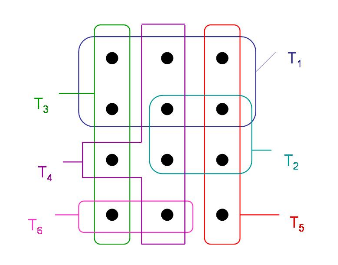
\includegraphics[width=0.4\textwidth]{Figures/set_cover.png}\centering
\end{figure}

Το ελάχιστο set cover είναι το σύνολο $S' = \{T_3, T_4, T_5\}$

\begin{figure}[H]
\caption{Minimum set cover example}
\centering
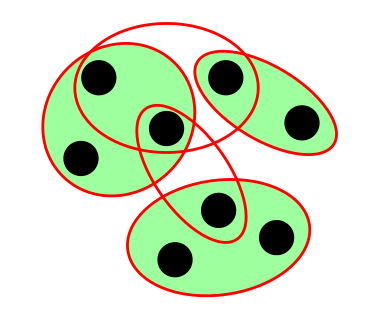
\includegraphics[width=0.4\textwidth]{Figures/min_set_cover.png}\centering
\end{figure}

%----------------------------------------------------------------------------------------
%	SECTION 2
%----------------------------------------------------------------------------------------

\section{NP-πληρότητα}

To set cover decision problem είναι ένα από τα 21 NP-πλήρης προβλήματα του Karp που αποδείχθηκε ότι είναι NP-πλήρης το 1972. Αυτό σημαίνει ότι ανήκει στην κλάση NP δηλαδή δεδομένου ενός σύμπαντος $U$, μιας συλλογής $S$ από υποσύνολα, ενός ακεραίου $k$ και μίας λύσης $S'$ η λύση αυτή μπορεί να επαληθευτεί σε πολυωνυμικό χρόνο όσον αφορά το μέγεθος των στοιχείων της εισόδου. Επίσης ανήκει και στην κλάση NP-hard. Αυτό οδήγησε στην ανάπτυξη προσεγγιστικών αλγορίθμων για την επίλυση του προβλήματος αυτού.


\section{Λύσεις}

\subsection{Πρόβλημα ακέραιου προγραμματισμού}

Το minimum set cover problem μπορεί να διατυπωθεί ως το ακόλουθο πρόβλημα ακέραιου προγραμματισμού

$$min\{\displaystyle\sum_{S\in{\mathcal{S}}} x_S\}$$ 
\centerline{subject to}
$$\displaystyle\sum_{S:e\in{\mathcal{S}}} x_S \geq{1}, \quad \forall e \in{\mathcal{U}}$$
$$ x_S \in{\{0, 1\}}$$

Επειδή το πρόβλημα ακέραιου προγραμματισμού είναι NP-hard χαλαρώνουμε τους περιορισμούς του προβλήματος για το $x_S$ και το ανάγουμε σε πρόβλημα γραμμικού προγραμματισμού το οποίο λύνεται σε πολυωνυμικό χρόνο. Έτσι καταλήγουμε στο πρόβλημα:

$$min\{\displaystyle\sum_{S\in{\mathcal{S}}} x_S\}$$ 
\centerline{subject to}
$$\displaystyle\sum_{S:e\in{\mathcal{S}}} x_S \geq{1}, \quad \forall e \in{\mathcal{U}}$$
$$ x_S \in{[0, 1]}$$

Επειδή το integrality gap αυτού του προβλήματος είναι το πολύ $\log{n}$ η χαλάρωση του δίνει factor-$\log{n}$ προσεγγιστικό αλγόριθμο.
Αν κάθε στοιχείο εμφανίζεται το πολύ σε ${\mathcal{F}}$ τότε μπορεί να βρεθεί λύση σε πολυωνυμικό χρόνο η οποία προσεγγίζει το βέλτιστο με παράγοντα ${\mathcal{F}}$ χρησιμοποιώντας το πρόβλημα γραμμικού προγραμματισμού.

\subsection{Άπληστος αλγόριθμος} 

Υπάρχει και ένας άπληστος αλγόριθμος για προσέγγιση σε πολυωνυμικό χρόνο ο οποίος διαλέγει τα σύνολα με έναν μόνο κανόνα: σε κάθε στάδιο διαλέγει το σύνολο που περιέχει τον μεγαλύτερο αριθμό από ακάλυπτα στοιχεία.

Αλγόριθμος:
\begin{enumerate}
\item $ C \leftarrow \emptyset$
\item While $ C \neq {\mathcal{U}} $ do
\begin{enumerate}
\item Find the set whose cost effectiveness is smallest, say $S_i$. \\
			Let $a = \frac{c(S_i)}{|S_i-C|}$. \\
			Pick $S_i$ and $\forall e \in{S_i - C}$, set $price(e) = a$.
\item $C \leftarrow S_i \cup C$
\end{enumerate}
\item Output $C$
\end{enumerate}

\section{Hitting set}
Το πρόβλημα set cover είναι ισοδύναμο με το πρόβλημα hitting set. Αν σε έναν διμερή γράφο το ένα σύνολο κόμβων ${\mathcal{U}}$ αντιπροσωπεύει τα υποσύνολα ${\mathcal{S}}$ του σύμπαντος, το άλλο σύνολο κόμβων ${\mathcal{V}}$ αντιπροσωπεύει τα στοιχεία του σύμπαντος και οι ακμές αντιπροσωπεύουν την συμπερίληψη ενός στοιχείου σε ένα σύνολο τότε βρίσκουμε τον ελάχιστο αριθμό κόμβων του συνόλου ${\mathcal{U}}$ που καλύπτει όλους τους κόμβους του συνόλου ${\mathcal{V}}$.

\section{Εφαρμογές}
IBM finds computer viruses (wikipedia) 
elements- 5000 known viruses 
sets- 9000 substrings of 20 or more consecutive bytes from viruses, not found in ‘good’ code 
A set cover of 180 was found.  It suffices to search 
for these 180 substrings to verify the existence of 
known computer viruses. 
Another example:  Consider General Motors needs to 
buy a certain amount of varied supplies and there are 
suppliers that offer various deals for different combina
tions of materials (Supplier A: 2 tons of steel + 500 tiles 
for \$x; Supplier B: 1 ton of steel + 2000 tiles for \$y; etc.).  You could use set covering to find the best way to 
get all the materials while minimizing cost
\chapter{Vertex cover problem} % Main chapter title

\label{Chapter2} % Change X to a consecutive number; for referencing this chapter elsewhere, use \ref{ChapterX}
\justify
To vertex cover ενός γράφου είναι ένα σύνολο κόμβων τέτοιο ώστε κάθε ακμή του γράφου είναι προσκείμενη σε τουλάχιστον ένα κόμβο του συνόλου αυτού. Το πρόβλημα εύρεσης του ελάχιστου vertex cover είναι κλασικό πρόβλημα στον τομέα της συνδυαστικής βελτιστοποίησης και της θεωρίας υπολογιστών και κλασικό παράδειγμα NP-hard προβλήματος βελτιστοποίησης. 
%----------------------------------------------------------------------------------------
%	SECTION 1
%----------------------------------------------------------------------------------------

\section{Διατύπωση}
Το vertex cover $V'$ ενός μη κατευθυντικού γράφου $G=(V,E)$ είναι ένα υποσύνολο του $V$ τέτοιο ώστε:
$$\forall uv \in{E} \Rightarrow u \in{V'} \lor v \in{V'}$$
Ένα τέτοιο σύνολο λέμε ό τι καλύπτει τις ακμές του $G$. Το ελάχιστο vertex cover ενός γράφου $G$ είναι το σύνολο $V'$ με τον μικρότερο αριθμό στοιχείων.


\begin{figure}[H]
\caption{Vertex cover}
\centering
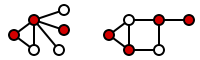
\includegraphics{Figures/vert_cover.png}\centering
\end{figure}

\begin{figure}[H]
\caption{Minimum vertex cover}
\centering
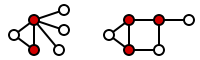
\includegraphics{Figures/min_vert_cover.png}\centering
\end{figure}

%----------------------------------------------------------------------------------------
%	SECTION 2
%----------------------------------------------------------------------------------------

\section{NP-πληρότητα}

Στη γενική περίπτωση το πρόβλημα vertex cover είναι NP-πλήρης οπότε είναι απίθανο να βρεθεί ακριβής αλγοριθμική λύση σε πολυωνυμικό χρόνο εκτός και αν P = NP. H NP-πληρότητα μπορεί να αποδειχθεί με υπαγωγή από το 3-SAT πρόβλημα ή από το Clique πρόβλημα. Σε ειδικές περιπτώσεις γράφων όμως μπορούν να βρεθούν πολυωνυμικοί αλγόριθμοι. Με εξαντλητική αναζήτηση το πρόβλημα μπορεί να λυθεί σε $2^{k}n^{O(1)}$ χρόνο, όπου k το μέγεθος του συνόλου και n ο αριθμός των κόμβων, το οποίο κάνει το πρόβλημα fixed-parameter tractable. Οπότε αν ενδιαφερόμαστε για μικρά k μπορούμε να επιλέξουμε αυτή τη μέθοδο και να έχουμε λύση σε πολυωνυμικό χρόνο.

\section{Λύσεις}

\subsection{Πρόβλημα ακέραιου προγραμματισμού}

Το minimum vertex cover problem μπορεί να διατυπωθεί ως το ακόλουθο πρόβλημα ακέραιου προγραμματισμού

$$min\{\displaystyle\sum_{u\in{V}} c(v)x_v\}$$ 
\centerline{subject to}
$$x_u + x_v \geq{1}, \quad \forall (u, v) \in{E}$$
$$ x_v \in{\{0, 1\}} \quad \forall v \in{V}$$

όπου $c : V \rightarrow {\boldsymbol{R}^+}$ μια συνάρτηση κόστους για τους κόμβους του γράφου.\\
Ο περιορισμός $$ x_v \in{\{0, 1\}} \quad \forall v \in{V}$$ σημαίνει ότι ένας κόμβος $v$ είτε ανήκει στο σύνολο $V'$ είτε όχι,
ενώ ο περιορισμός $$x_u + x_v \geq{1}, \quad \forall (u, v) \in{E}$$ σημαίνει ότι για κάθε ακμή τουλάχιστον ένας κόμβος της πρέπει να ανήκει στο σύνολο $V'$
και η συνάρτηση που θέλουμε να ελαχιστοποιήσουμε είναι το αθροισμά των βαρών των κόμβων που βρίσκονται στο σύνολο $V'$ δηλαδή τα $v$ εκείνα για τα οποία το $x_v$ είναι $1$.

\subsubsection{Χαλάρωση}

Επειδή το πρόβλημα ακέραιου προγραμματισμού είναι NP-hard χαλαρώνουμε τους περιορισμούς του προβλήματος για το $x_v$ και το ανάγουμε σε πρόβλημα γραμμικού προγραμματισμού το οποίο λύνεται σε πολυωνυμικό χρόνο. Έτσι καταλήγουμε στο πρόβλημα:

$$min\{\displaystyle\sum_{u\in{V}} c(v)x_v\}$$ 
\centerline{subject to}
$$x_u + x_v \geq{1}, \quad \forall (u, v) \in{E}$$
$$ x_v \in [0,1], \quad \forall v \in{V}$$

\subsubsection{Integrality gap}
Το integrality gap ενός προβλήματος γραμμικού προγραμματισμού που έχει προκύψει από τη χαλάρωση ενός προβλήματος ακέραιου προγραμματισμού ορίζεται το 

$$\sup_{I} \frac{OPT(I)}{OPT_f(I)}$$

όπου $OPT(I)$ είναι η βέλτιστη λύση του προβλήματος ακέραιου προγραμματισμού και $OPT_f(I)$ είναι η βέλτιστη λύση του προβλήματος γραμμικού προγραμματισμού.\\

Το integrality gap του παραπάνω προβλήματος είναι $2$ οπότε η χαλάρωση του δίνει έναν factor-$2$ προσεγγιστικό αλγόριθμο. Επίσης η γραμμική χαλάρωση του προβλήματος είναι half-integral, δηλάδη υπάρχει βέλτιστη λύση στην οποία $x_v \in{\{0, \frac{1}{2}, 1\}}$	

\subsubsection{Half-integrality}

Το παραπάνω πρόβλημα ακέραιου προγραμματισμού έχει αλλή μια πολύ ενδιαερουσα ιδιότητα: κάθε εφικτή λύση που δεν είναι half-integral δηλαδή $x_v \in{\{0, \frac{1}{2}, 1\}} \quad \forall x_v \in V'$ είναι κυτρός συνδυασμός δυό εφικτών λύσεων και άρα δεν είναι λύση ακραίου σημείου.\\

Απόδειξη:\\
Έστω το σύνολο των κόμβων για το οποίο η λύση $\boldsymbol{x}$ δεν είναι half-integral, χωρίζουμε αυτό το σύνολο :

$$V_{+}=\Big\{v \Big| \frac{1}{2} < x_v < 1\Big\}, \quad V_{-}=\Big\{v \Big| 0 < x_v < \frac{1}{2} \Big\}$$

Για κάποιο $\varepsilon > 0$ ορίζουμε τις ακόλουθες λύσεις: 

$$y_v = \begin{cases}
x_v + \varepsilon, \quad x_v \in V_{+}\\
x_v - \varepsilon, \quad x_v \in V_{-}\\
x_v , \quad \text{otherwise}\\
\end{cases}$$

και 

$$z_v = \begin{cases}
x_v - \varepsilon, \quad x_v \in V_{+}\\
x_v + \varepsilon, \quad x_v \in V_{-}\\
x_v , \quad \text{otherwise}\\
\end{cases}$$

Έχουμε ότι $V_{+}\cup V_{-} \neq \emptyset$ οπότε το $\boldsymbol{x}$ είναι διάφορο του $\boldsymbol{y}$ και $\boldsymbol{z}$, και για αρκετά μικρό $\varepsilon$
έχουμε $0 \geq y, z \geq 1$. Επίσης ισχύει $x = \frac{1}{2} (y + z)$.
Αν:
\begin{enumerate}
\item
$$x_v + x_u > 1 \implies 
\begin{cases}
(x_i + x_j) - (y_i + y_j) \leq 2\varepsilon\\
(x_i + x_j) - (z_i + z_j) \leq 2\varepsilon\\
\end{cases}
$$
\centering Και για αρκετά μικρό $\varepsilon$ έχουμε 
$$ 
\begin{cases}
y_i + y_j \geq 1\\
z_i + z_j \geq 1\\
\end{cases}
$$
\item


\end{enumerate}

άρα η λύση $\boldsymbol{x}$ δεν είναι λύση ακραίου σημείου.

\subsection{Προσεγγιστικοί αλγόριθμοι} 

Έχουν αναπτυχθεί πολλές παραλλαγές προσεγγιστικών αλγορίθμων που λύνουν το συγκεκριμένο πρόβλημα. Ο πιο απλός αλγόριθμος είναι factor-2  προσεγγιστικός και αναπτύχθηκε ανεξάρτητα από τους Fanica Gavril και τον Μιχάλη Γιαννακάκη. Η γενική ιδέα είναι η εξής: σε κάθε επανάληψη διαλέγει μια ακμή και εισάγει και τα δύο άκρα $(u, v)$ της στο vertex cover $V'$, και αφαιρεί από το σύνολο των ακμών κάθε ακμή που είναι προσκείμενη είτε στον κόμβο $u$ είτε στον $v$ μέχρι να μείνει το κενό σύνολο.\\
Αλγόριθμος:
\begin{enumerate}
\item $ V' \leftarrow \emptyset $
\item $ E' \leftarrow E$
\item While $ E' \neq {\emptyset} $ do
\begin{enumerate}[a)]
\item let (u, v) be an arbitrary edge of $E'$
\item $V' \leftarrow V' \cup \{u,v\}$
\item remove from $E'$ every edge incident on either u or v 
\end{enumerate}
\item Output $V'$
\end{enumerate}

Ο αλγόριθμος αυτός τρέχει σε χρόνο $O(|V| + |E|)$. Όσον αφορά τον παράγοντα προσέγγγισης του αλγορίθμου φαίνεται εύκολα ότι για το σύνολο των ακμών που επιλέγονται στο βήμα $\alpha')$ ισχύει 
$$|V^{*}| \geq |A|$$ 
αφού το σύνολο $Α$ δεν περιέχει προσκείμενες ακμές και επειδή το σύνολο $V'$ που επιστρέφει ο αλγόριθμος περιέχει και τις δυο κορυφές των ακμών που επιλέγει έχουμε 
$$|V'| = 2|A|$$ 
οπότε 
$$|V'| \leq 2|V^{*}|$$ 

Έχουν αναπτυχθεί και άλλοι προσεγγίστικοι αλγόριθμοι με καλύτερο παράγοντα προσέγγισης, όπως $2-\Theta\Big(\frac{1}{\sqrt{\log{|V|}}}\Big)$ αλλά δεν έχει βρεθεί καλύτερος αλγόριθμος σταθερού προσεγγιστικού παράγοντα. Το minimum vertex cover πρόβλημα είναι $APX-$πλήρης δηλαδή δεν μπορεί να προσεγγιστεί αυθαίρετα καλά αν δεν ισχύει $P=NP$. Οι Dinur και Safra απέδειξαν ότι το πρόβλημα δε μπορεί να προσεγγιστεί με παράγοντα μικρότερο του $1.3606$ για έναν αρκετά μεγάλο γράφο αν δεν ισχύει $P=NP$, επίσης αν ισχυέι η εικασία unique games τότε το πρόβλημα δεν μπορεί να προσεγγιστεί με σταθερό πράγοντα μικρότερο του $2$. 

\chapter{Ειδικές περιπτώσεις} % Main chapter title

\label{Chapter3} % Change X to a consecutive number; for referencing this chapter elsewhere, use \ref{ChapterX}
Το πρόβλημα vertex cover παρόλο που είναι NP-πλήρης στη γενική περίπτωση σε κάποιες ειδικές περιπτώσεις γράφων είναι δυνατό να λυθεί σε πολυωνυμικό χρόνο. Παρακάτω παραθέτονται κάποιες από αυτές τις ειδικές περιπτώσεις και ορισμένες λύσεις και πορίσματα.
%----------------------------------------------------------------------------------------
%	SECTION 1
%----------------------------------------------------------------------------------------

\section{Bigraphs}

\subsection{Εισαγωγικές έννοιες}

\begin{enumerate}
\item
Διμερής γράφοι:\\
Οι διμερείς γράφοι είναι ειδικές περιπτώσεις γράφων που οι κόμβοι τους μπορούν να χωριστούν σε δύο ανεξάρτητα σύνολα $\mathcal{U}$ και $\mathcal{V}$ έτσι ώστε κάθε ακμή να ενώνει ένα κόμβο του $\mathcal{U}$ με έναν κόμβο του $\mathcal{V}$. 
\item
Matching:\\
Δεδομένου ενός γράφου $G=(V,E)$ ονομάζουμε matching $Μ$ στον $G$ ένα σύνολο μη γειτονικών ακμών, δηλαδή ακμές που δεν είναι προσκείμενες στον ίδιο κόμβο. Μέγιστο matching ονομάζουμε το σύνολο με τον μέγιστο αριθμό ακμών.
\end{enumerate}
\begin{figure}[H]
\caption{Matching example}
\centering
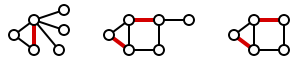
\includegraphics{Figures/match.png}\centering
\end{figure}

\begin{figure}[H]
\caption{Maximum matching example}
\centering
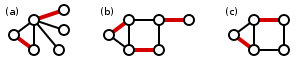
\includegraphics{Figures/max_match.png}\centering
\end{figure}

\subsection{Θεώρημα Konig}

Σε αυτό το είδος γράφων βρίσκει εφαρμογή το θεώρημα του Konig το οποίο αναφέρει πως για κάθε διμερή γράφο $G=(V,E)$ ισχύει $\nu(G) = \tau(G)$ όπου\\
$\nu(G) := $ maximum size of a matching in G,\\
$\tau(G) := $ minimum size of a vertex cover in G.

\subsection{Απόδειξη}
\justify
Έστω ένας διμερής γράφος $G = (L, R, E)$ και ένα μέγιστο ταίριασμα $M$. Τότε επειδή κανένας κόμβος ενός vertex cover δεν μπορεί να καλύπτει περισσότερες από δύο ακμές του συνόλου $M$ (διαφορετικά δεν θα ήταν ταίριασμα), ένα vertex cover μεγέθους $|M|$ θα είναι το ελάχιστο vertex cover.\\
Για να δημιουργήσουμε ένα τέτοιο vertex cover, έστω $U$ το σύνολο των μη ταιριασμένων κόμβων του $L$, και $Z$ το σύνολο των ακμών που είτε είναι στο $U$ είτε συνδέονται με αυτό μέσω εναλλακτικών μονοπατιών (alternating paths). Τότε το σύνολο $V' = (L \setminus Z) \cup (R \cap Z)$ είναι ένα vertex cover. 

\subsection{Συμπεράσματα}

Οπότε χρησιμοποιώντας τον αλγόριθμο Hopcroft-Karp, ο οποίος βρίσκει ένα μέγιστο ταίριασμα σε ένα διμερή γράφο σε χρόνο $O(|E| \sqrt{|V|})$, μπορούμε έπειτα να υπολογίσουμε το σύνολο $V'$ αποδοτικά.
Επίσης για όλους τους γράφους ισχύει 
$$ \max_{\text{matching M}} |M| \leq  \min_{\text{vertex cover U}} |U| \leq 2 \cdot \Big( \max_{\text{mathing M}} |M|\Big)$$
\begin{figure}[H]
\caption{Maximum matching - minimum vertex cover example}
\centering
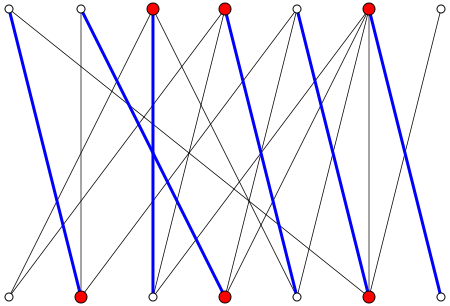
\includegraphics[width=0.4\textwidth]{Figures/KonigTheo.png}\centering
\end{figure}
%----------------------------------------------------------------------------------------
%	SECTION 2
%----------------------------------------------------------------------------------------

\section{Tree graphs}
Για δένδρα υπάρχει ένας άπληστος αλγόριθμος που βρίσκει το ελάχιστο vertex cover σε πολυωνυμικό χρόνο.

\subsection{Εισαγωγικές έννοιες}
Ένα δένδρο είναι ένας μη κατευθυντικός γράφος $G=(V,E)$ που είναι συνεκτικός και δεν έχει κύκλους.

\subsection{Αλγόριθμος}
Η βασική ιδέα του αλγορίθμου είναι η εξής: χρησιμοποιώντας την αναζήτηση πρώτα σε βάθος βρίσκουμε όλα τα φύλλα του δένδρου και έπειτα για κάθε φύλλο επιλέγουμε τον πατέρα του, έπειτα επιλέγουμε κάθε εσωτερικό κόμβο που τα παιδιά του δεν έχουν επιλεχθεί μέχρι να μην υπάρχουν άλλοι κόμβοι να επιλεχθούν.

\begin{figure}[H]
\caption{Vertex cover in tree example}
\centering
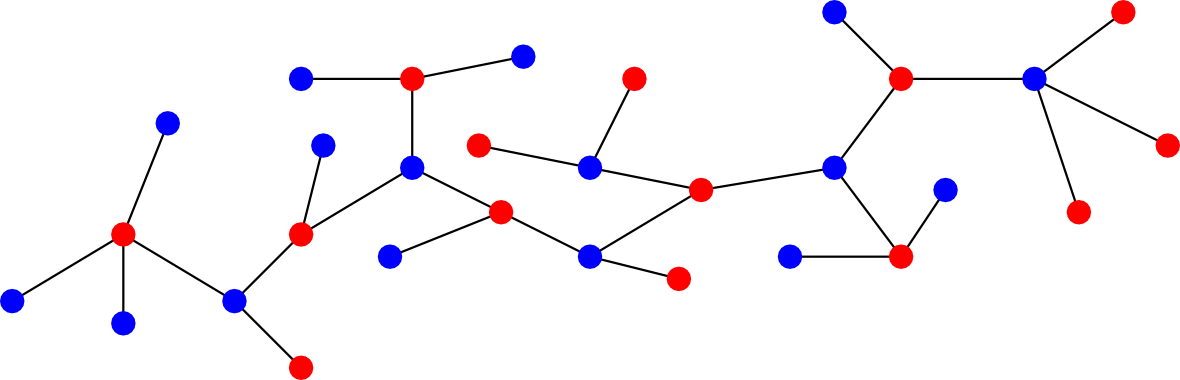
\includegraphics[width=0.5\textwidth]{Figures/vc_tree.png}\centering
\end{figure}

%----------------------------------------------------------------------------------------
%	SECTION 3
%----------------------------------------------------------------------------------------

\section{Hypergraphs}
\subsection{Εισαγωγικές έννοιες}
Υπεργράφος είναι μια γενίκευση του γράφου όπου μια ακμή μπορεί να συνδέσει περισσότερους από έναν κόμβους. Πιο αυστηρά ένας υπεργράφος $H$ είναι ένα ζευγάρι $H=(X,E)$ όπου $X$ είναι ένα σύνολο του οποίου τα στοιχεία είναι οι κόμβοι και $E$ είναι ένα σύνολο αποτελούμενο από μη κενά υποσύνολα του $X$ και ονομάζονται υπερακμές. 

Το πρόβλημα εύρεσης του vertex cover ενός hypergraph ονομάζεται transversal, και είναι ισοδύναμο με το hitting set.

%----------------------------------------------------------------------------------------
%	SECTION 4
%----------------------------------------------------------------------------------------

\section{Δυικά προβλήματα}

Το πρόβλημα vertex cover συνδέται και με άλλα συνδυαστικά προβλήματα σε γράφους μέσα από κάποιες δυικές σχέσεις. Κάποια από αυτά τα προβλήματα αναφέρονται παρακάτω.

\subsection{Clique}
Ένα clique ενός μη κατευθυντικού γράφου $G=(V,E)$ είναι ένα υποσύνολο των ακμών $C \subseteq V$ τέτοιο ώστε όλοι οι κόμβοι του να είναι γειτονικοί ανά δύο.\\
Δεδομένου ενός μη κατευθυντικού γράφου $G=(V,E)$ ορίζουμε το συμπλήρωμα του ως $\overline{G} = (V, \overline{E})$ όπου $\overline{E} = \{(u,v):u,v \in{V}, u \neq v, (u,v) \notin{E}\}$, τότε αν υπάρχει ένα clique $C$ στον $\overline{G}$ το $V \setminus C$ είναι ένα vertex cover του $G$.

\begin{figure}[H]
\caption{Clique example}
\centering
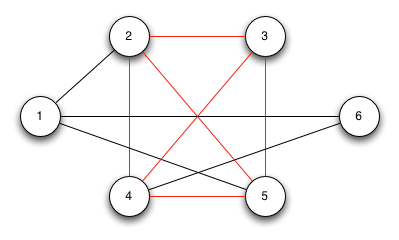
\includegraphics[width=0.4\textwidth]{Figures/VertexClique.png}\centering
\end{figure}

\subsection{Independent set}
Το independent set ενός γράφου είναι ένα σύνολο των κόμβων του οι οποίοι δεν είναι γειτονικοί ανά δύο. Το πρόβλημα εύρεσης του μέγιστου independent σετ είναι ένα κλασικό NP-hard πρόβλημα βελτιστοποίησης. Το πρόβλημα αυτό σχετίζεται με το πρόβλημα vertex cover καθώς για κάθε independent set ενός γράφου το συμπλήρωμα του είναι ένα vertex cover για αυτόν τον γράφο.	

\begin{figure}[H]
\caption{Independent set example}
\centering
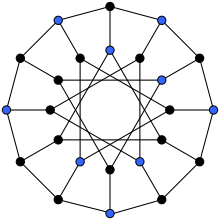
\includegraphics[width=0.3\textwidth]{Figures/indep_set.png}\centering
\end{figure}

\chapter{Εφαρμογές} % Main chapter title

\label{Chapter4} % Change X to a consecutive number; for referencing this chapter elsewhere, use \ref{ChapterX}

\section{Παραδείγματα εφαρμογών}
Το πρόβλημα εύρεσης του vertex cover ενός γράφου βρίσκει εφαρμογές σε διαφόρων ειδών προβλήματα τα οποία μπορεί εκ πρώτης όψεος να μην έχουν κάποιο κοινό γνώρισμα αλλά μπορούν να αναχθούν σε προβλήματα εύρεσης ενός ελαχίστου υποσύνολου το οποίο να "καλύπτει" ένα άλλο σύνολο.

\par{
Κάποια απλά παραδείγματα εφορμογής είναι τα εξής:

Έστω ότι θέλουμε να τοποθετήσουμε τροχονόμους στο οδικό δίκτυο μια πόλης, το πρόβλημα που προκύπτει είναι πώς μπορούμε να τοποθετήσουμε τους τροχονόμους με βέλτιστο τρόπο ώστε να χρησιμοποιήσουμε τον ελάχιστο αριθμό τροχονόμων που να "καλύπτουν" όλους τους δρόμους της πόλης. 
Αυτό το πρόβλημα μπορεί να μοντελοποιηθεί ως ένα minimum vertex cover πρόβλημα όπου οι ακμές είναι οι δρόμοι της πόλης και οι τροχονόμοι οι κόμβοι.
}
\par{
Άλλο παρόμοιο παράδειγμα: έστω ότι θέλουμε να τοποθετήσουμε κάμερες σε ένα κτήριο, πως μπορούμε να τοποθετήσουμε τις κάμερες με βέλτιστο τρόπο ώστε να έχουμε τον ελάχιστο αριθμό καμερών που να καλύπτουν όλους τους χώρους του κτηρίου; Και αυτό είναι ένα πρόβλημα που μπορεί να μοντελοποιηθεί ως minimum vertex cover πρόβλημα.
}

\par{
Ένα άλλο πρακτικό παράδειγμα είναι στην δυναμική ανίχνευση race conditions. Αν έχουμε ένα νήμα το οποίο γράφει σε μία θέσης μνήμης και έπειτα ένα άλλο νήμα προσπαθήσει να γράψει στην ίδια θέση μνήμης σημαίνει ότι κρατάει ένα lock για συγκεκριμένη θέση. Έτσι μπορούμε να ορίσουμε δύο σύνολα ένα το οποίο περιέχει τα νήματα και ένα που περιέχει τα locks για τις θέσεις μνήμης και ακμές που να αντιπροσωπεύουν την ιδιοκτησία κάποιου lock από ένα νήμα. Τότε το minimum hitting set αντιπροσωπεύει τον ελάχιστο σύνολο απο locks που είναι race-free. Το οποίο χρησιμοποιείται στη συνέχεια για την εξάλειψη περιττών εγγραφών.\cite{DataRaces}
}

\par{
Τέλος ένα παράδειγμα από τον τομέα της υπολογιστικής βιοχημείας όπου σε πολλά προβλήματα χρειάζεται η εξάλειψη συγκρούσεων μεταξύ αλληλουχιών ενός δείγματος. Το πρόβλημα μοντελοποείται ως γράφος όπου οι κόμβοι αντιπροσωπεύουν τις αλληλουχίες του δείγματος και οι ακμές τις μεταξύ τους συγκρούσεις. Ο στόχος είναι να αφαιρεθούν όσον το δυνατόν λιγότεροι κόμβοι ώστε να μην υπάρχουν καθόλου συγκρούσεις στον γράφο.\cite{SNP}
}

\section{Υλοποίηση}

{
\centering
\usemintedstyle{monokai}
\inputminted[
frame=lines,
framesep=2mm,
baselinestretch=1.2,
bgcolor=darkgray,
fontsize=\footnotesize,
linenos
]{cpp}{Figures/code.cpp}
}\\

\justify
Η παραπάνω συνάρτηση υλοποιεί τον προσεγγιστικό αλγόριθμο που παρουσιάστηκε στη παράγραφο 2.3.2. Η συνάρτηση καλείται σε ένα γράφο που αποτελείται από ένα σύνολο ακμών (edges) και ένα σύνολο κόμβων (vertices) και επιστρέφει ένα σύνολο κόμβων (vertex\_cover) που αντιπροσωπεύει το vertex cover του γράφου. Η συνάρτηση remove\_edge χρησιμοποιείται για να διαγράφει από ένα σύνολο ακμών όλες τις ακμές που είναι προσκύμενες σε ένα συγκεκριμένο κόμβο. Παρακάτω φαίνονται τα αποτελέσματα του αλγορίθμου, με κόκκινο συμβολίζονται οι κόμβοι που ανήκουν στο vertex cover του γράφου ενώ με άσπρο αυτοί που δεν ανήκουν.

\begin{figure}[H]
\caption{Vertex cover implementation example 1, 7 vertices}
\centering
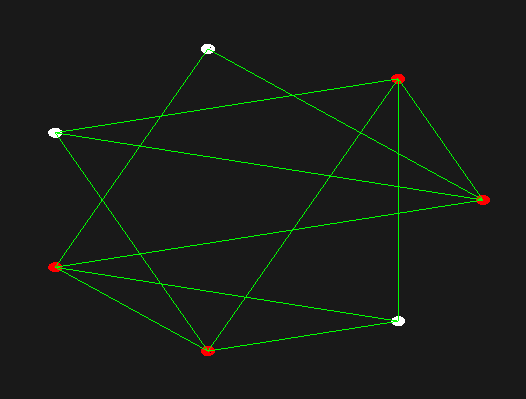
\includegraphics[width=0.6\textwidth]{Figures/code.png}\centering
\end{figure}

Με χρήση της βιβλιοθήκης Cbc που αποτελεί μέρος του COIN-OR project, και υλοποιεί αλγορίθμους για επίλυση προβλημάτων ακέραιου προγραμματισμού, μοντελοποιούμε το vertex cover problem σε πρόβλημα ακεραιού  προγραμματισμού. Φορτώνουμε τον πίνακα γειτνίασης του παραπάνω γράφου.

\begin{figure}[H]
\caption{Adjacency matrix}
\centering
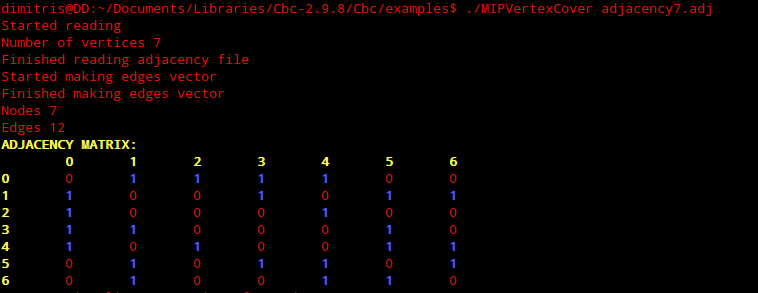
\includegraphics[width=1.1\textwidth]{Figures/adjac.png}\centering
\end{figure}

Και έπειτα τον χρησιμοποιούμε για να βρούμε τους περιορισμούς του προβλήματος.


\begin{figure}[H]
\caption{System Equations}
\centering
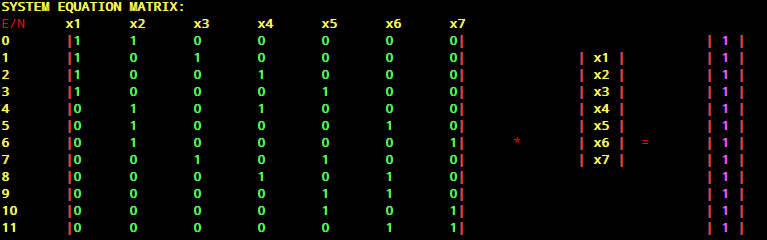
\includegraphics[width=1.1\textwidth]{Figures/sys.png}\centering
\end{figure}


\begin{figure}[H]
\caption{Solution}
\centering
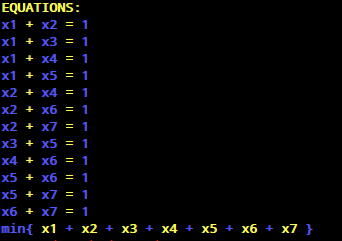
\includegraphics[width=0.6\textwidth]{Figures/const.png}\centering
\end{figure}

Και τέλος η λύση του προβλήματος δείχνει ότι επιλέγοντε 4 κόμβοι (αυτοί για τους οποίους η τιμή είναι 1) για το vertex cover όπως βρήκε και ο άπληστος αλγόριθμος.

\begin{figure}[H]
\caption{Vertex cover implementation example 1, 7 vertices}
\centering
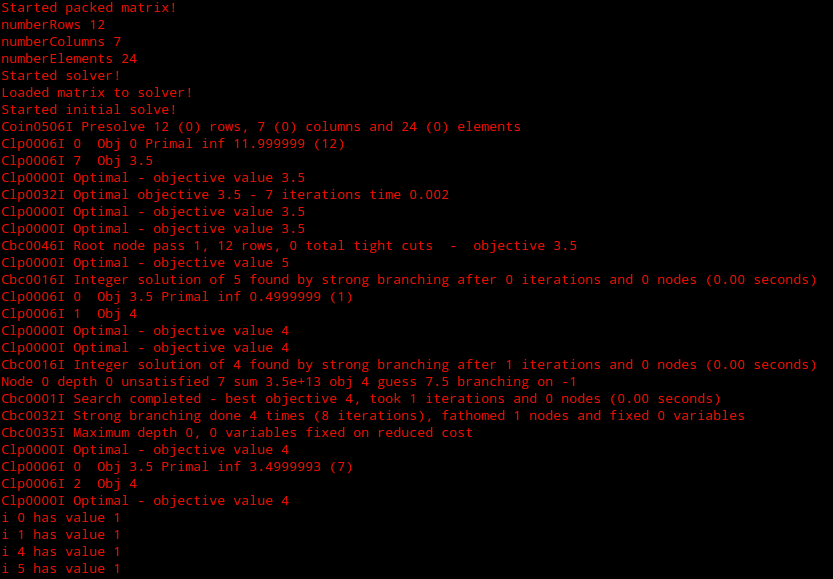
\includegraphics[width=1.3\textwidth]{Figures/sol_int.png}\centering
\end{figure}

Ενώ η χαλάρωση του προβλήματος και η λύση του με γραμμικό προγραμματισμό δίνει σε όλες τις μεταβλητές την τιμή 0.5, οπότε σύμφωνα με τα προηγούμενα θα πρέπει να επιλέξουμε όλους τους κόμβους στο vertex cover.

\begin{figure}[H]
\caption{Vertex cover implementation example 1, 7 vertices}
\centering
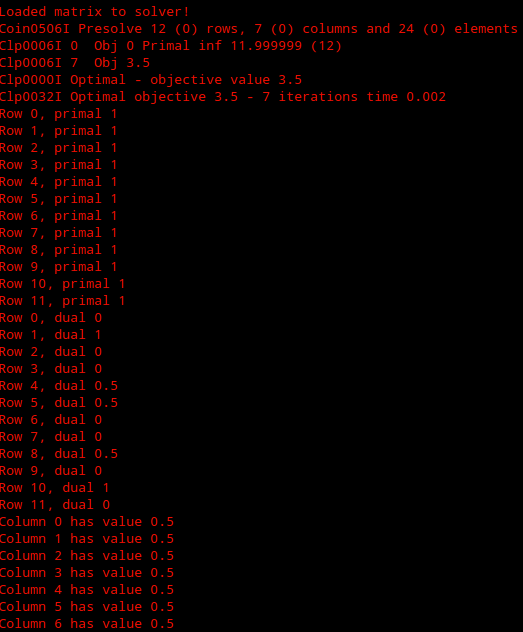
\includegraphics[width=1.1\textwidth]{Figures/sol_frac.png}\centering
\end{figure} 

%----------------------------------------------------------------------------------------
%	THESIS CONTENT - APPENDICES
%----------------------------------------------------------------------------------------

%\appendix % Cue to tell LaTeX that the following "chapters" are Appendices

% Include the appendices of the thesis as separate files from the Appendices folder
% Uncomment the lines as you write the Appendices

%% Appendix A

\chapter{Appendix Title Here} % Main appendix title

\label{AppendixA} % For referencing this appendix elsewhere, use \ref{AppendixA}

Write your Appendix content here.
%\include{Appendices/AppendixB}
%\include{Appendices/AppendixC}

%----------------------------------------------------------------------------------------
%	BIBLIOGRAPHY
%----------------------------------------------------------------------------------------

\printbibliography[heading=bibintoc]

%----------------------------------------------------------------------------------------

\end{document}  
